% Options for packages loaded elsewhere
% Options for packages loaded elsewhere
\PassOptionsToPackage{unicode}{hyperref}
\PassOptionsToPackage{hyphens}{url}
\PassOptionsToPackage{dvipsnames,svgnames,x11names}{xcolor}
%
\documentclass[
  letterpaper,
  DIV=11,
  numbers=noendperiod]{scrartcl}
\usepackage{xcolor}
\usepackage{amsmath,amssymb}
\setcounter{secnumdepth}{5}
\usepackage{iftex}
\ifPDFTeX
  \usepackage[T1]{fontenc}
  \usepackage[utf8]{inputenc}
  \usepackage{textcomp} % provide euro and other symbols
\else % if luatex or xetex
  \usepackage{unicode-math} % this also loads fontspec
  \defaultfontfeatures{Scale=MatchLowercase}
  \defaultfontfeatures[\rmfamily]{Ligatures=TeX,Scale=1}
\fi
\usepackage{lmodern}
\ifPDFTeX\else
  % xetex/luatex font selection
\fi
% Use upquote if available, for straight quotes in verbatim environments
\IfFileExists{upquote.sty}{\usepackage{upquote}}{}
\IfFileExists{microtype.sty}{% use microtype if available
  \usepackage[]{microtype}
  \UseMicrotypeSet[protrusion]{basicmath} % disable protrusion for tt fonts
}{}
\makeatletter
\@ifundefined{KOMAClassName}{% if non-KOMA class
  \IfFileExists{parskip.sty}{%
    \usepackage{parskip}
  }{% else
    \setlength{\parindent}{0pt}
    \setlength{\parskip}{6pt plus 2pt minus 1pt}}
}{% if KOMA class
  \KOMAoptions{parskip=half}}
\makeatother
% Make \paragraph and \subparagraph free-standing
\makeatletter
\ifx\paragraph\undefined\else
  \let\oldparagraph\paragraph
  \renewcommand{\paragraph}{
    \@ifstar
      \xxxParagraphStar
      \xxxParagraphNoStar
  }
  \newcommand{\xxxParagraphStar}[1]{\oldparagraph*{#1}\mbox{}}
  \newcommand{\xxxParagraphNoStar}[1]{\oldparagraph{#1}\mbox{}}
\fi
\ifx\subparagraph\undefined\else
  \let\oldsubparagraph\subparagraph
  \renewcommand{\subparagraph}{
    \@ifstar
      \xxxSubParagraphStar
      \xxxSubParagraphNoStar
  }
  \newcommand{\xxxSubParagraphStar}[1]{\oldsubparagraph*{#1}\mbox{}}
  \newcommand{\xxxSubParagraphNoStar}[1]{\oldsubparagraph{#1}\mbox{}}
\fi
\makeatother


\usepackage{longtable,booktabs,array}
\usepackage{calc} % for calculating minipage widths
% Correct order of tables after \paragraph or \subparagraph
\usepackage{etoolbox}
\makeatletter
\patchcmd\longtable{\par}{\if@noskipsec\mbox{}\fi\par}{}{}
\makeatother
% Allow footnotes in longtable head/foot
\IfFileExists{footnotehyper.sty}{\usepackage{footnotehyper}}{\usepackage{footnote}}
\makesavenoteenv{longtable}
\usepackage{graphicx}
\makeatletter
\newsavebox\pandoc@box
\newcommand*\pandocbounded[1]{% scales image to fit in text height/width
  \sbox\pandoc@box{#1}%
  \Gscale@div\@tempa{\textheight}{\dimexpr\ht\pandoc@box+\dp\pandoc@box\relax}%
  \Gscale@div\@tempb{\linewidth}{\wd\pandoc@box}%
  \ifdim\@tempb\p@<\@tempa\p@\let\@tempa\@tempb\fi% select the smaller of both
  \ifdim\@tempa\p@<\p@\scalebox{\@tempa}{\usebox\pandoc@box}%
  \else\usebox{\pandoc@box}%
  \fi%
}
% Set default figure placement to htbp
\def\fps@figure{htbp}
\makeatother





\setlength{\emergencystretch}{3em} % prevent overfull lines

\providecommand{\tightlist}{%
  \setlength{\itemsep}{0pt}\setlength{\parskip}{0pt}}



 


\KOMAoption{captions}{tableheading}
\makeatletter
\@ifpackageloaded{caption}{}{\usepackage{caption}}
\AtBeginDocument{%
\ifdefined\contentsname
  \renewcommand*\contentsname{Table of contents}
\else
  \newcommand\contentsname{Table of contents}
\fi
\ifdefined\listfigurename
  \renewcommand*\listfigurename{List of Figures}
\else
  \newcommand\listfigurename{List of Figures}
\fi
\ifdefined\listtablename
  \renewcommand*\listtablename{List of Tables}
\else
  \newcommand\listtablename{List of Tables}
\fi
\ifdefined\figurename
  \renewcommand*\figurename{Figure}
\else
  \newcommand\figurename{Figure}
\fi
\ifdefined\tablename
  \renewcommand*\tablename{Table}
\else
  \newcommand\tablename{Table}
\fi
}
\@ifpackageloaded{float}{}{\usepackage{float}}
\floatstyle{ruled}
\@ifundefined{c@chapter}{\newfloat{codelisting}{h}{lop}}{\newfloat{codelisting}{h}{lop}[chapter]}
\floatname{codelisting}{Listing}
\newcommand*\listoflistings{\listof{codelisting}{List of Listings}}
\makeatother
\makeatletter
\makeatother
\makeatletter
\@ifpackageloaded{caption}{}{\usepackage{caption}}
\@ifpackageloaded{subcaption}{}{\usepackage{subcaption}}
\makeatother
\usepackage{bookmark}
\IfFileExists{xurl.sty}{\usepackage{xurl}}{} % add URL line breaks if available
\urlstyle{same}
\hypersetup{
  pdftitle={The New Classical Approach},
  pdfauthor={Adapted by Dr Camilo Calderon},
  colorlinks=true,
  linkcolor={blue},
  filecolor={Maroon},
  citecolor={Blue},
  urlcolor={Blue},
  pdfcreator={LaTeX via pandoc}}


\title{The New Classical Approach}
\author{Adapted by Dr Camilo Calderon}
\date{}
\begin{document}
\maketitle

\renewcommand*\contentsname{Table of contents}
{
\hypersetup{linkcolor=}
\setcounter{tocdepth}{3}
\tableofcontents
}

\section{Introduction}\label{introduction}

The New Classical approach extends monetarist skepticism about policy
fine-tuning by sharpening the mechanism through which policy affects
real outcomes. The key shift is from short-run money illusion under
adaptive expectations (Friedman's framework) to model-consistent
forecasting under rational expectations, which removes systematic policy
surprises and eliminates systematic real effects of monetary policy.

\subsection{Expectations and the rational expectations
revolution}\label{expectations-and-the-rational-expectations-revolution}

\subsubsection{Adaptive expectations}\label{adaptive-expectations}

Adaptive expectations operate as a trial-and-error forecasting rule
where agents update forecasts using past observed outcomes:

Price expectations: \(E_{t-1}P_t = f(P_{t-1}, P_{t-2}, ...)\)

A common error-correction form is:
\[\pi_t^e = \pi_{t-1}^e + \lambda(\pi_{t-1} - \pi_{t-1}^e), \quad 0 < \lambda \le 1.\]

Adaptive expectations permit systematic forecast errors during regime
changes, creating temporary money illusion and thus temporary real
effects.

\subsubsection{Rational expectations}\label{rational-expectations}

Rational expectations are defined by three criteria: (i) forecasts use
the true economic model (agents know the economy's structure), (ii)
forecasts condition on all available information, and (iii) forecast
errors are purely random---systematic errors are eliminated.

In classical formulation: expectations are ``the same as the predictions
of the relevant economic theory,'' and the economy does not waste
information.

Model-consistent forecasting: \[E_{t-1}P_t = E(P_t \mid I_{t-1}),\]
where \(I_{t-1}\) is the information set at time \(t-1\).

If workers have access to unbiased forecasts, predictable policy loses
its ability to manipulate perceived real wages and thus loses its
ability to shift real output, even in the short run.

\section{The New Classical model of output and
prices}\label{the-new-classical-model-of-output-and-prices}

\subsection{Lucas aggregate supply and aggregate
demand}\label{lucas-aggregate-supply-and-aggregate-demand}

The New Classical model consists of two equations: Lucas supply (LAS)
and aggregate demand (AD).

\textbf{Lucas aggregate supply (LAS):} Output deviates from potential
only when the price level differs from expectations:
\[Y_t^s - Y^* = \kappa(P_t - E_{t-1}P_t).\]

Lucas (1972) derives this in a market-clearing framework with optimizing
agents.

Interpretation: - If \(P_t > E_{t-1}P_t\): firms perceive relative-price
gains, supply rises (\(Y_t^s > Y^*\)) - If \(P_t = E_{t-1}P_t\): output
at potential (\(Y_t^s = Y^*\)) - If \(P_t < E_{t-1}P_t\): output below
potential (\(Y_t^s < Y^*\))

The parameter \(\kappa\) measures supply responsiveness:
\(\partial Y_t / \partial(P_t - E_{t-1}P_t) = \kappa\).

\textbf{Aggregate demand (AD):} In log form:
\[Y_t^d = \gamma + M_t - P_t,\] where \(M_t\) is nominal money and
\(\gamma\) captures exogenous demand shifts.

Agents know structural parameters \(\gamma\), \(\kappa\), and natural
output \(Y^*\).

\subsection{\texorpdfstring{Solving the model: the role of
\(\kappa\)}{Solving the model: the role of \textbackslash kappa}}\label{solving-the-model-the-role-of-kappa}

Equilibrium: \(Y_t^s = Y_t^d = Y_t\). Combining LAS and AD:

\begin{enumerate}
\def\labelenumi{\arabic{enumi}.}
\item
  Under rational expectations: \[E_{t-1}Y_t = Y^*.\]
\item
  Output deviations depend only on monetary surprises:
  \[Y_t - Y^* = \frac{\kappa}{1+\kappa}(M_t - E_{t-1}M_t).\]
\item
  Price surprises scale with monetary surprises:
  \[P_t - E_{t-1}P_t = \frac{1}{1+\kappa}(M_t - E_{t-1}M_t).\]
\end{enumerate}

Interpretation: larger \(\kappa\) means output responds more, prices
respond less; smaller \(\kappa\) reverses this. The Lucas supply slope
(P on vertical axis, Y horizontal) is proportional to \(1/\kappa\).

When policy is volatile, agents discount price movements as noise (``boy
who cried wolf''), lowering effective \(\kappa\) and steepening LAS.

\section{Monetary policy
implications}\label{monetary-policy-implications}

\subsection{The monetary policy ineffectiveness
proposition}\label{the-monetary-policy-ineffectiveness-proposition}

With rational expectations and market clearing, \emph{systematic and
predictable} monetary policy has \textbf{no real effect}, even
short-run. Predictable policy is incorporated into expectations,
shifting prices, not real outcomes.

Formally, if \(M_t = E_{t-1}M_t\) (policy is forecastable):
\[Y_t - Y^* = 0.\]

\subsection{Systematic rules versus random
disturbances}\label{systematic-rules-versus-random-disturbances}

Sharp distinction: (i) predictable rule-like policy vs.~(ii) random
disturbances.

Money supply process: \[M_t = (1 + g_M)M_{t-1} + u_t,\] where \(u_t\) is
white noise (\(E_{t-1}u_t = 0\)).

Then: \(E_{t-1}M_t = (1 + g_M)M_{t-1}\), so \(M_t - E_{t-1}M_t = u_t\).

Output deviations: \[Y_t - Y^* = \frac{\kappa}{1+\kappa}u_t.\]

\textbf{Only randomness affects output.} Predictable money growth
affects the price level, not real activity.

\subsection{Why deliberate unpredictability is not
recommended}\label{why-deliberate-unpredictability-is-not-recommended}

The model should not justify randomness. Two reasons:

\begin{enumerate}
\def\labelenumi{\arabic{enumi}.}
\tightlist
\item
  Random policies produce recessions and booms equally (negative \(u_t\)
  as likely as positive).
\item
  High volatility changes behaviour: agents discount price signals,
  steepening LAS (lower effective \(\kappa\), higher price response).
\end{enumerate}

This logic explains modern central-bank transparency: policy is more
effective when expectations are anchored and communication reduces
unnecessary uncertainty.

\section{Exceptions and policy
extensions}\label{exceptions-and-policy-extensions}

Two important exceptions: monetary policy can stabilise real activity
under rational expectations if key assumptions are relaxed.

\subsection{Asymmetric information and real
shocks}\label{asymmetric-information-and-real-shocks}

If productivity shocks drive cycles and the central bank forecasts a
negative shock before the private sector, it can expand policy in
advance to stabilise output (at higher prices).

This fits the New Classical framework because the CB has an
informational advantage, creating a price surprise from the public's
perspective.

Compatible with real-business-cycle reasoning: technology/productivity
shocks drive cycles.

\subsection{Long-term nominal wage contracts and
stabilisation}\label{long-term-nominal-wage-contracts-and-stabilisation}

In many economies, nominal wages are fixed by multi-year contracts. Even
if demand shocks are anticipated, monetary policy can offset them
because some nominal wages cannot adjust immediately---rigidity creates
stabilisation scope.

This aligns with Fischer (1977): under wage rigidity, monetary rules
interact with shock propagation even under rational expectations.

Under symmetric information (no CB informational advantage),
stabilisation works best for demand shocks; supply-side stabilisation
requires informational asymmetry.

\subsection{Lucas critique and
credibility}\label{lucas-critique-and-credibility}

The \textbf{Lucas critique}: policy-effect estimates from historical
relationships are unreliable if decision rules shift with the regime.
This motivates structural, microfounded models.

If agents form expectations rationally, \textbf{commitment and
credibility} shape outcomes through expectations. Rules, strategy
statements, and transparent communication are policy tools.

Time-inconsistency literature: policy is strategic interaction with
rational agents. Discretionary optimisation can backfire because
promises today are not optimal tomorrow (after expectations set).
Central to rules-versus-discretion analysis.

\section{Modern evidence and
applications}\label{modern-evidence-and-applications}

\subsection{Measuring policy
surprises}\label{measuring-policy-surprises}

New Classical model disturbance: \(M_t - E_{t-1}M_t\). Modern empirical
work isolates surprise components using high-frequency financial data.

Recent IMF working paper: dataset of monetary policy shocks for 21
advanced and 8 emerging economies (2000--2022), using daily changes in
interest rate swap rates around central bank announcements to identify
unexpected policy shocks to the rate path. Maps directly to model:
unexpected shocks are the empirical analogue of \(u_t\).

\subsection{Credibility and anchored expectations in
practice}\label{credibility-and-anchored-expectations-in-practice}

New Classical analysis makes credibility central. Modern CBs frame
policy as expectations management.

Federal Reserve: publishing its ``Statement on Longer-Run Goals and
Monetary Policy Strategy'' helps the public understand the
framework---matters for transparency, accountability, and effectiveness.

ECB (2021 strategy): symmetric 2\% medium-term inflation aim; notes that
effective lower bound can require ``especially forceful or persistent''
measures, including transitory inflation above target.

IMF research: better-anchored expectations → less persistent inflation
responses to shocks, reinforcing New Classical emphasis on credibility
and expectations formation.

\subsection{Policy regime episodes}\label{policy-regime-episodes}

\textbf{Bank of Japan:} reference timeline documents unconventional
regimes from late 1990s onward (ZIRP 1999, QE from 2001). Explicitly
lists ``policy duration effect (forward guidance)'' as part of ZIRP---an
expectations-management concept compatible with New Classical theory.

Japan's 2024 framework change: QQE with yield curve control and negative
rates judged to have ``fulfilled their roles,'' shifting back to
short-rate guidance---regime transition where expectations and
credibility matter.

\textbf{ECB (June 2014):} introducing negative deposit facility rate
(--0.10\% effective June 11, 2014) illustrates how rules change when
constraints bind and why expectation formation is central to
transmission.

\textbf{COVID-19 emergency actions:} central banks reacted with
large-scale measures for market functioning and macro stabilisation,
showing regime and expectations logic when short rates are constrained.

\subsection{Comparative framework: mechanisms and
applications}\label{comparative-framework-mechanisms-and-applications}

\begin{longtable}[]{@{}
  >{\raggedright\arraybackslash}p{(\linewidth - 4\tabcolsep) * \real{0.2558}}
  >{\raggedright\arraybackslash}p{(\linewidth - 4\tabcolsep) * \real{0.2558}}
  >{\raggedright\arraybackslash}p{(\linewidth - 4\tabcolsep) * \real{0.4884}}@{}}
\toprule\noalign{}
\begin{minipage}[b]{\linewidth}\raggedright
Mechanism
\end{minipage} & \begin{minipage}[b]{\linewidth}\raggedright
Prediction
\end{minipage} & \begin{minipage}[b]{\linewidth}\raggedright
Modern illustration
\end{minipage} \\
\midrule\noalign{}
\endhead
\bottomrule\noalign{}
\endlastfoot
Systematic, predictable policy & If anticipated, shifts \(E_{t-1}P_t\)
one-for-one; \(Y_t \approx Y^*\) & Fed and ECB strategy statements
anchor expectations through transparency. \\
Unanticipated shocks & Only surprise component drives
\(P_t - E_{t-1}P_t\), hence \(Y_t - Y^*\) & IMF high-frequency dataset
(2000--2022) identifies unexpected policy shocks at announcements. \\
Policy volatility & Agents discount price signals; LAS steepens (lower
effective \(\kappa\)) & CBs prefer predictable reaction functions over
crisis-era surprise moves. \\
Wage contracts & Nominal rigidity reopens stabilisation, even under
rational expectations & BoE COVID interventions supported market
functioning and prevented tightening. \\
Informational advantage & CB with better real-shock information can
offset systematically & BoJ forward guidance and regime design link to
RBC-style productivity shocks. \\
\end{longtable}

\section{Figures}\label{figures}

\textbf{Figure 1. Lucas aggregate supply: output deviates from potential
only when P differs from expected price.} If expectations are correct,
output remains at potential.

\begin{verbatim}
Warning: package 'ggplot2' was built under R version 4.4.3
\end{verbatim}

\begin{verbatim}
Warning in geom_point(aes(x = Y_star, y = E_P), color = "black", size = 3): All aesthetics have length 1, but the data has 200 rows.
i Please consider using `annotate()` or provide this layer with data containing
  a single row.
\end{verbatim}

\begin{figure}

\centering{

\pandocbounded{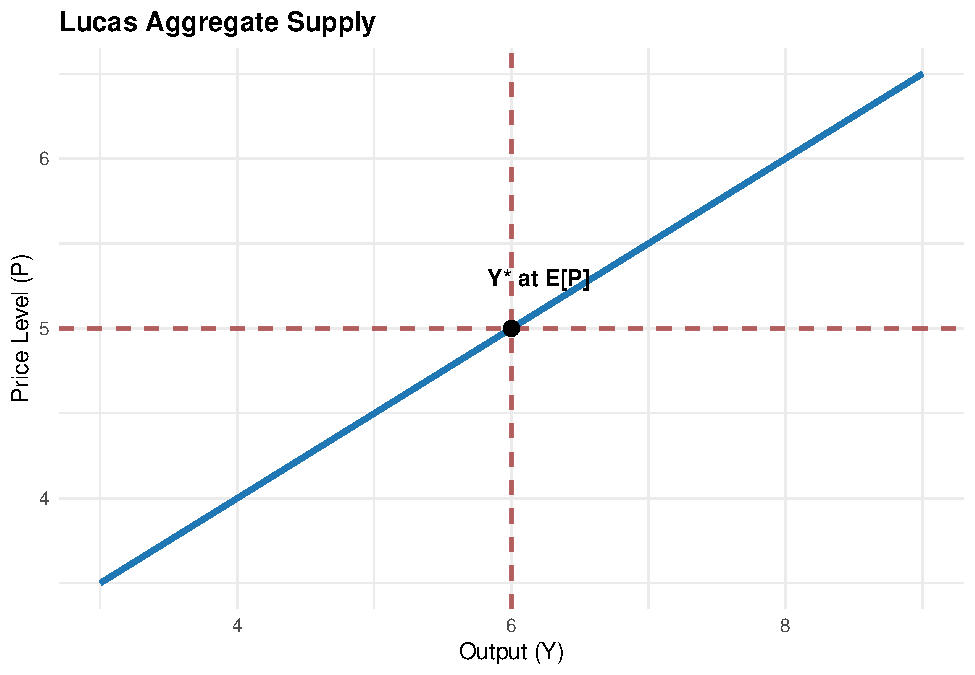
\includegraphics[keepaspectratio]{topic5reading_files/figure-pdf/fig-lucas-supply-1.pdf}}

}

\caption{\label{fig-lucas-supply}Lucas Aggregate Supply:
\(Y_t - Y^* = \kappa(P_t - E_{t-1}P_t)\)}

\end{figure}%

\textbf{Figure 2. Predictable versus unpredictable monetary policy.} A
predictable rise in money shifts AD and LAS upward (via expectations);
equilibrium stays at \(Y^*\). An unpredictable rise shifts AD without
shifting LAS initially; equilibrium moves along LAS with \(Y\) above
\(Y^*\).

\begin{verbatim}
Warning in geom_point(aes(x = Y_eq_1, y = P_eq_1), color = "darkred", size = 3, : All aesthetics have length 1, but the data has 450 rows.
i Please consider using `annotate()` or provide this layer with data containing
  a single row.
\end{verbatim}

\begin{verbatim}
Warning in geom_point(aes(x = Y_eq_2, y = P_eq_2), color = "darkgreen", : All aesthetics have length 1, but the data has 450 rows.
i Please consider using `annotate()` or provide this layer with data containing
  a single row.
\end{verbatim}

\begin{figure}

\centering{

\pandocbounded{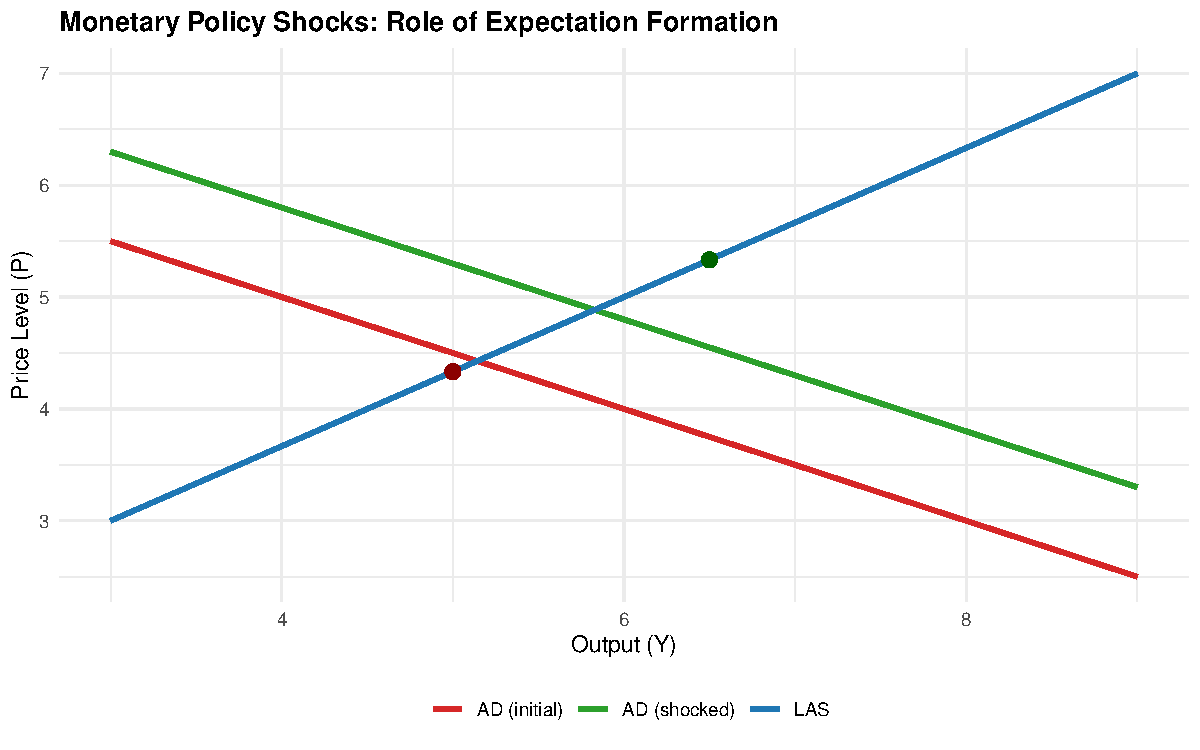
\includegraphics[keepaspectratio]{topic5reading_files/figure-pdf/fig-predictable-unpredictable-1.pdf}}

}

\caption{\label{fig-predictable-unpredictable}Policy predictability
determines whether output effects are temporary.}

\end{figure}%

\textbf{Figure 3. Policy volatility reduces supply responsiveness via
information effects.} Greater policy volatility lowers the informational
content of observed price movements. Agents cannot distinguish
relative-price signals from aggregate noise, reducing supply response
(lower \(\kappa\)) and steepening LAS.

\begin{figure}

\centering{

\pandocbounded{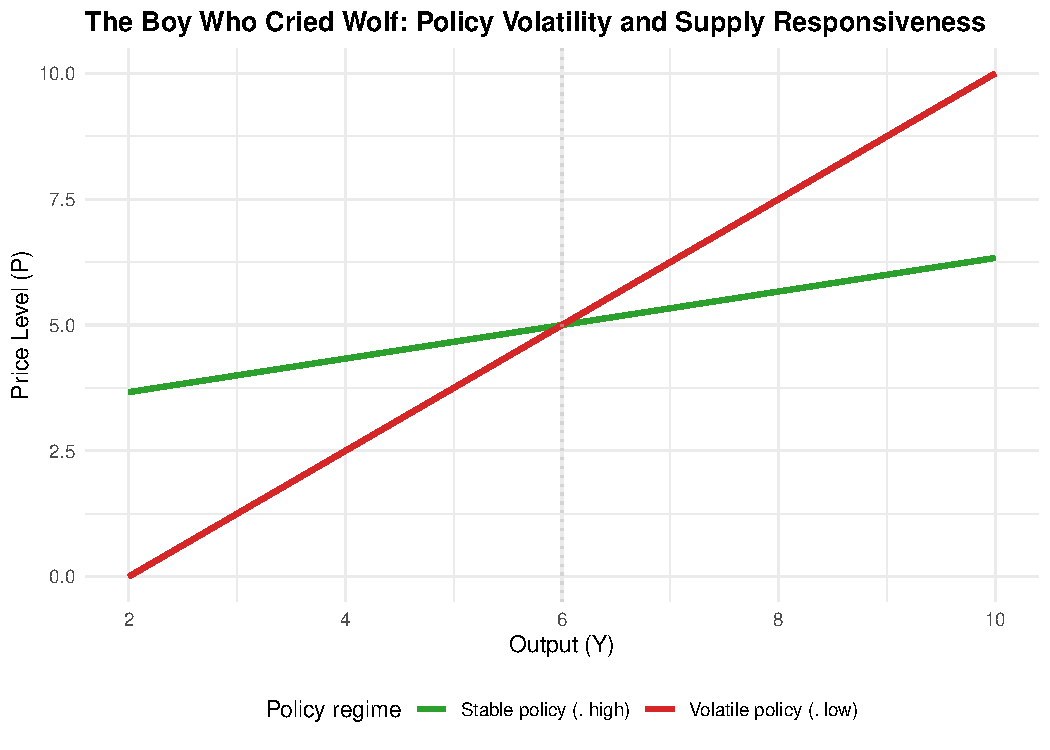
\includegraphics[keepaspectratio]{topic5reading_files/figure-pdf/fig-volatility-effect-1.pdf}}

}

\caption{\label{fig-volatility-effect}Higher policy volatility steepens
Lucas supply through information effects.}

\end{figure}%

\section{Problem questions}\label{problem-questions}

\begin{enumerate}
\def\labelenumi{\arabic{enumi}.}
\item
  In the LAS equation \(Y_t - Y^* = \kappa(P_t - E_{t-1}P_t)\),
  interpret every term economically. Why does the model predict
  \(E_{t-1}Y_t = Y^*\) under rational expectations?
\item
  Show that equilibrium output deviations are
  \(Y_t - Y^* = (\kappa/(1+\kappa))(M_t - E_{t-1}M_t)\). What happens as
  \(\kappa \to 0\)? As \(\kappa \to \infty\)?
\item
  Explain why ``random policy can move output'' is not an argument for
  deliberate policy randomness. Explain using both (i) sign symmetry of
  shocks and (ii) the ``boy who cried wolf'' information mechanism.
\item
  Describe the asymmetric-information exception: what must be true about
  the central bank's information set relative to the private sector's
  for systematic stabilisation to operate under rational expectations?
\item
  Explain Fischer's wage-contract critique: why can anticipated monetary
  policy offset demand shocks when only part of the economy's wages are
  flexible?
\item
  Using high-frequency monetary policy shock data, explain how
  researchers operationalise ``policy surprises.'' Why is this relevant
  to the New Classical policy-ineffectiveness result?
\end{enumerate}

\section{References}\label{references}

Fischer, S. (1977). Long-term contracts, rational expectations, and the
optimal money supply rule. \emph{Journal of Political Economy}, 85(1),
191--205.

International Monetary Fund. (2024). A new dataset of high-frequency
monetary policy shocks (Working Paper 2024/224).

International Monetary Fund. (2018). Expectations' anchoring and
inflation persistence (Working Paper 2018/280).

Lucas, R. E., Jr.~(1972). Expectations and the neutrality of money.
\emph{Journal of Economic Theory}, 4(2), 103--124.

Muth, J. F. (1961). Rational expectations and the theory of price
movements. \emph{Econometrica}, 29(3), 315--335.

Nerlove, M. (1958). Adaptive expectations and cobweb phenomena.
\emph{The Quarterly Journal of Economics}, 72(2), 227--240.

Prescott, E. C. (1986). Theory ahead of business cycle measurement.
\emph{Quarterly Review} / Federal Reserve Bank of Minneapolis (Staff
Report 102).

Sargent, T. J., \& Wallace, N. (1976). Rational expectations and the
theory of economic policy. \emph{Journal of Monetary Economics}, 2(2),
169--183.

Sargent, T. J., \& Wallace, N. (1975). ``Rational'' expectations, the
optimal monetary instrument, and the optimal money supply rule.
\emph{Journal of Political Economy}, 83(2), 241--254.

European Central Bank. (2014). ECB introduces a negative deposit
facility interest rate (Press release, 5 June).

European Central Bank. (2021). The ECB's monetary policy strategy
statement.

Bank of England. (2020). Bank Rate reduced to 0.1\% and asset purchases
increased by £200bn (Monetary Policy Summary, 19 March).

Bank of Japan. (2024). Changes in the Monetary Policy Framework (19
March).

Bank of Japan. (n.d.). Unconventional Monetary Policy Measures from the
Late 1990s.

Federal Reserve Board. (2025). Statement on Longer-Run Goals and
Monetary Policy Strategy.

\section{The New Classical model of output and
prices}\label{the-new-classical-model-of-output-and-prices-1}

\subsection{Lucas aggregate supply and aggregate
demand}\label{lucas-aggregate-supply-and-aggregate-demand-1}

The New Classical model consists of two equations: Lucas supply (LAS)
and aggregate demand (AD).

\textbf{Lucas aggregate supply (LAS):} Output deviates from potential
only when the price level differs from expectations:
\[Y_t^s - Y^* = \kappa(P_t - E_{t-1}P_t).\]

Lucas (1972) derives this in a market-clearing framework with optimizing
agents.

Interpretation: - If \(P_t > E_{t-1}P_t\): firms perceive relative-price
gains, supply rises (\(Y_t^s > Y^*\)) - If \(P_t = E_{t-1}P_t\): output
at potential (\(Y_t^s = Y^*\)) - If \(P_t < E_{t-1}P_t\): output below
potential (\(Y_t^s < Y^*\))

The parameter \(\kappa\) measures supply responsiveness:
\(\partial Y_t / \partial(P_t - E_{t-1}P_t) = \kappa\).

\textbf{Aggregate demand (AD):} In log form:
\[Y_t^d = \gamma + M_t - P_t,\] where \(M_t\) is nominal money and
\(\gamma\) captures exogenous demand shifts.

Agents know structural parameters \(\gamma\), \(\kappa\), and natural
output \(Y^*\).

\subsection{\texorpdfstring{Solving the model: the role of
\(\kappa\)}{Solving the model: the role of \textbackslash kappa}}\label{solving-the-model-the-role-of-kappa-1}

Equilibrium: \(Y_t^s = Y_t^d = Y_t\). Combining LAS and AD:

\begin{enumerate}
\def\labelenumi{\arabic{enumi}.}
\item
  Under rational expectations: \[E_{t-1}Y_t = Y^*.\]
\item
  Output deviations depend only on monetary surprises:
  \[Y_t - Y^* = \frac{\kappa}{1+\kappa}(M_t - E_{t-1}M_t).\]
\item
  Price surprises scale with monetary surprises:
  \[P_t - E_{t-1}P_t = \frac{1}{1+\kappa}(M_t - E_{t-1}M_t).\]
\end{enumerate}

Interpretation: larger \(\kappa\) means output responds more, prices
respond less; smaller \(\kappa\) reverses this. The Lucas supply slope
(P on vertical axis, Y horizontal) is proportional to \(1/\kappa\).

When policy is volatile, agents discount price movements as noise (``boy
who cried wolf''), lowering effective \(\kappa\) and steepening LAS.

\section{Monetary policy
implications}\label{monetary-policy-implications-1}

\subsection{The monetary policy ineffectiveness
proposition}\label{the-monetary-policy-ineffectiveness-proposition-1}

With rational expectations and market clearing, \emph{systematic and
predictable} monetary policy has \textbf{no real effect}, even
short-run. Predictable policy is incorporated into expectations,
shifting prices, not real outcomes.

Formally, if \(M_t = E_{t-1}M_t\) (policy is forecastable):
\[Y_t - Y^* = 0.\]

\subsection{Systematic rules versus random
disturbances}\label{systematic-rules-versus-random-disturbances-1}

Sharp distinction: (i) predictable rule-like policy vs.~(ii) random
disturbances.

Money supply process: \[M_t = (1 + g_M)M_{t-1} + u_t,\] where \(u_t\) is
white noise (\(E_{t-1}u_t = 0\)).

Then: \(E_{t-1}M_t = (1 + g_M)M_{t-1}\), so \(M_t - E_{t-1}M_t = u_t\).

Output deviations: \[Y_t - Y^* = \frac{\kappa}{1+\kappa}u_t.\]

\textbf{Only randomness affects output.} Predictable money growth
affects the price level, not real activity.

\subsection{Why deliberate unpredictability is not
recommended}\label{why-deliberate-unpredictability-is-not-recommended-1}

The model should not justify randomness. Two reasons:

\begin{enumerate}
\def\labelenumi{\arabic{enumi}.}
\tightlist
\item
  Random policies produce recessions and booms equally (negative \(u_t\)
  as likely as positive).
\item
  High volatility changes behaviour: agents discount price signals,
  steepening LAS (lower effective \(\kappa\), higher price response).
\end{enumerate}

This logic explains modern central-bank transparency: policy is more
effective when expectations are anchored and communication reduces
unnecessary uncertainty.

\section{Exceptions and policy
extensions}\label{exceptions-and-policy-extensions-1}

Two important exceptions: monetary policy can stabilise real activity
under rational expectations if key assumptions are relaxed.

\subsection{Asymmetric information and real
shocks}\label{asymmetric-information-and-real-shocks-1}

If productivity shocks drive cycles and the central bank forecasts a
negative shock before the private sector, it can expand policy in
advance to stabilise output (at higher prices).

This fits the New Classical framework because the CB has an
informational advantage, creating a price surprise from the public's
perspective.

Compatible with real-business-cycle reasoning: technology/productivity
shocks drive cycles.

\subsection{Long-term nominal wage contracts and
stabilisation}\label{long-term-nominal-wage-contracts-and-stabilisation-1}

In many economies, nominal wages are fixed by multi-year contracts. Even
if demand shocks are anticipated, monetary policy can offset them
because some nominal wages cannot adjust immediately---rigidity creates
stabilisation scope.

This aligns with Fischer (1977): under wage rigidity, monetary rules
interact with shock propagation even under rational expectations.

Under symmetric information (no CB informational advantage),
stabilisation works best for demand shocks; supply-side stabilisation
requires informational asymmetry.

\subsection{Lucas critique and
credibility}\label{lucas-critique-and-credibility-1}

The \textbf{Lucas critique}: policy-effect estimates from historical
relationships are unreliable if decision rules shift with the regime.
This motivates structural, microfounded models.

If agents form expectations rationally, \textbf{commitment and
credibility} shape outcomes through expectations. Rules, strategy
statements, and transparent communication are policy tools.

Time-inconsistency literature: policy is strategic interaction with
rational agents. Discretionary optimisation can backfire because
promises today are not optimal tomorrow (after expectations set).
Central to rules-versus-discretion analysis.

\section{Modern evidence and real-world
examples}\label{modern-evidence-and-real-world-examples}

\subsection{Measuring policy
surprises}\label{measuring-policy-surprises-1}

In the New Classical model, the disturbance term is
\(M_t - E_{t-1}M_t\). Modern empirical work isolates \emph{surprise
components} of policy announcements using high-frequency financial
market data.

A recent IMF working paper constructs a dataset of monetary policy
shocks for 21 advanced economies and 8 emerging markets (2000--2022)
using daily changes in interest rate swap rates around central bank
announcements to identify unexpected shocks to the policy path. This
maps directly onto the model's object: an unexpected policy shock is the
empirical analogue of \(u_t\) in the money-growth process.

\subsection{Credibility and anchored
expectations}\label{credibility-and-anchored-expectations}

New Classical analysis makes credibility and expectations central.
Modern central banks explicitly frame policy as expectations management.

The Federal Reserve explains that publishing its ``Statement on
Longer-Run Goals and Monetary Policy Strategy'' helps the public
understand the policy framework, which matters for transparency,
accountability, and effectiveness.

The ECB's 2021 strategy statement emphasises a symmetric 2\% medium-term
inflation aim and explicitly notes that the effective lower bound can
require ``especially forceful or persistent'' measures, potentially
including a transitory period of inflation moderately above target.

IMF research provides evidence that better-anchored expectations are
associated with less persistent inflation responses to shocks,
reinforcing the New Classical emphasis on credibility and expectations
formation.

\subsection{Policy regime episodes}\label{policy-regime-episodes-1}

The Bank of Japan reference timeline documents major unconventional
regimes from the late 1990s onward (ZIRP from 1999, QE from 2001, and
later phases). It explicitly lists policy duration effect (forward
guidance) as part of ZIRP---an expectations-management concept
compatible with New Classical thinking.

Japan's 2024 framework change statement explains that QQE with yield
curve control and negative rates were judged to have fulfilled their
roles, with a shift back to guiding the short-term interest rate as the
primary tool.

For the euro area, the ECB's June 2014 press release introducing a
negative deposit facility rate provides a canonical policy regime
expansion example: the ECB cut the deposit facility rate to \(-0.10\%\)
effective June 11, 2014.

During COVID-19, emergency actions show how central banks reacted to
extraordinary shocks with large-scale measures that were partly about
market functioning and partly about macro stabilisation.

\section{Problem questions}\label{problem-questions-1}

\begin{enumerate}
\def\labelenumi{\arabic{enumi}.}
\item
  In the LAS equation \(Y_t - Y^* = \kappa(P_t - E_{t-1}P_t)\),
  interpret every term economically. Why does the model predict
  \(E_{t-1}Y_t = Y^*\) under rational expectations?
\item
  Show that equilibrium output deviations are
  \(Y_t - Y^* = (\kappa/(1+\kappa))(M_t - E_{t-1}M_t)\). What happens as
  \(\kappa \to 0\)? What happens as \(\kappa \to \infty\)?
\item
  Explain why ``random policy can move output'' is not an argument for
  deliberate policy randomness. Explain using both (i) the sign symmetry
  of shocks and (ii) the ``boy who cried wolf'' mechanism.
\item
  Describe the asymmetric-information exception: what must be true about
  the central bank's information set relative to the private sector's
  for systematic stabilisation to operate under rational expectations?
\item
  Explain the wage-contract critique: why can anticipated monetary
  policy offset demand shocks when only part of the economy's wages are
  flexible?
\item
  Using high-frequency monetary policy shock data from modern empirical
  work, explain how researchers operationalise ``policy surprises.'' Why
  is this relevant to the New Classical policy-ineffectiveness result?
\end{enumerate}

\section{References}\label{references-1}

Fischer, S. (1977). Long-term contracts, rational expectations, and the
optimal money supply rule. \emph{Journal of Political Economy}, 85(1),
191--205.

International Monetary Fund. (2024). A new dataset of high-frequency
monetary policy shocks (Working Paper 2024/224).

Lucas, R. E., Jr.~(1972). Expectations and the neutrality of money.
\emph{Journal of Economic Theory}, 4(2), 103--124.

Muth, J. F. (1961). Rational expectations and the theory of price
movements. \emph{Econometrica}, 29(3), 315--335.

Prescott, E. C. (1986). Theory ahead of business cycle measurement.
\emph{Quarterly Review} / Federal Reserve Bank of Minneapolis (Staff
Report 102).

Sargent, T. J., \& Wallace, N. (1976). Rational expectations and the
theory of economic policy. \emph{Journal of Monetary Economics}, 2(2),
169--183.

European Central Bank. (2014). ECB introduces a negative deposit
facility interest rate (Press release, 5 June).

European Central Bank. (2021). The ECB's monetary policy strategy
statement.

Bank of England. (2020). Bank Rate reduced to 0.1\% and asset purchases
increased by £200bn (Monetary Policy Summary, 19 March).

Bank of Japan. (2024). Changes in the Monetary Policy Framework (19
March).

Bank of Japan. (n.d.). Unconventional Monetary Policy Measures from the
Late 1990s.




\end{document}
